% !TEX root = ../main.tex
\section{Introduction}\label{sec:introduction}

Barkeshli, Douglas, and Freedman~\cite{BDF2026} organize mathematical reasoning into a directed hypergraph whose vertices are propositions and whose hyperedges are inference rules, each connecting $p$ inputs to $q$ outputs.  They develop depth functions and inductive closure in the context of topological quantum field theory, but leave open the question of how to instantiate their framework on a concrete proof system.  Their structural hypergraph $\mathcal{S}$ contains all well-formed expressions, the universal proof hypergraph $\mathcal{U} \subset \mathcal{S}$ contains provable propositions, and the human mathematics $\mathcal{H} \subset \mathcal{U}$ contains what has been proved so far (Figure~\ref{fig:bdf-framework}).

CIC provides a direct instantiation.  Each sub-expression of the Calculus of Inductive Constructions is both a vertex and a hyperedge: \texttt{app} connects two children (width~1), \texttt{forallE} connects two children (width~1), \texttt{letE} connects three (width~2), and leaf nodes (\texttt{bvar}, \texttt{sort}, \texttt{const}, \texttt{lit}) are atoms (width~0).  Constructor arity determines width; expression nesting determines depth.  The depth filtration $A^{(0)} \subseteq A^{(1)} \subseteq \cdots$ stabilizes on any finite set of expressions, and nerves involved in reference cycles are precisely those excluded from the filtration.  These structural properties follow from the CIC grammar without additional axioms.

Making this hypergraph content-addressable, replacing name-based identity with hash-based identity, adds automatic deduplication.  In a traditional expression tree, \texttt{Const ``Nat''} appearing ten times in a proof term creates ten separate nodes.  In the content-addressed hypergraph, it is one nerve referenced ten times.  Since CIC typing rules reference declarations by key but never inspect the key's structure, type-checking is invariant under this substitution: the same parameterized kernel accepts or rejects the same declarations regardless of whether keys are strings or hashes.

This paper implements the above in Lean~4.  GenericKernel is a 400-line CIC kernel parameterized over a key type \texttt{Key}.  Instantiating at \texttt{Key = String} produces TreeKernel; instantiating at \texttt{Key = UInt64} produces NerveKernel.  NerveKernel adds a Merkle-style content hash (\texttt{String.hash}, producing \texttt{UInt64}) and a decomposition function Shatter that converts each expression tree into a set of content-addressed nerves.  Three theorems proved via \texttt{native\_decide} confirm that both instantiations succeed on a concrete environment of 15 declarations from \texttt{Nat} through \texttt{Nat.add\_comm}, producing environments of equal size.  Shatter decomposes those 15 declarations from 825 tree nodes into 280 nerves (66\% deduplication).  A separate Theory module formalizes the AstroNerve and AstroNet axioms with Mathlib, proving depth filtration stabilization and the cycle characterization of unstaged nerves.

\begin{figure}[H]
\centering
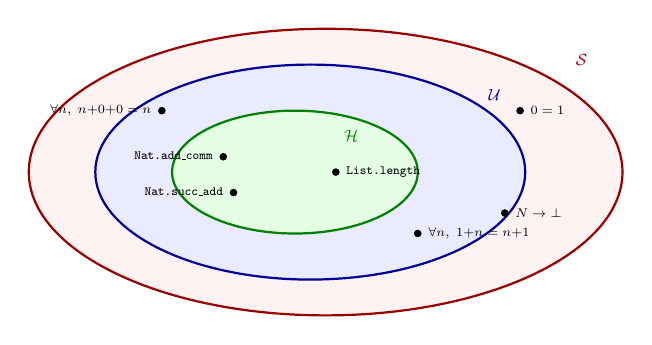
\begin{tikzpicture}[scale=0.65, every node/.style={transform shape},
  nd/.style={circle, fill=black, inner sep=1.5pt},
  expr/.style={font=\scriptsize\ttfamily},
  lbl/.style={font=\scriptsize, gray}
]
% --- Nested regions ---
\draw[thick, draw=red!60!black, fill=red!5] (0,0) ellipse (5.8cm and 2.8cm);
\draw[thick, draw=blue!60!black, fill=blue!8] (-0.3,0) ellipse (4.2cm and 2.1cm);
\draw[thick, draw=green!50!black, fill=green!10] (-0.6,0) ellipse (2.4cm and 1.2cm);
\node[font=\small, text=red!60!black] at (5.0, 2.2) {$\mathcal{S}$};
\node[font=\small, text=blue!60!black] at (3.3, 1.5) {$\mathcal{U}$};
\node[font=\small, text=green!50!black] at (0.5, 0.7) {$\mathcal{H}$};

% --- H: human-proved theorems ---
\node[nd] (h1) at (-2.0, 0.3) {};
\node[expr, left] at (h1.west) {\strut Nat.add\_comm};
\node[nd] (h2) at (-1.8, -0.4) {};
\node[expr, left] at (h2.west) {\strut Nat.succ\_add};
\node[nd] (h3) at (0.2, 0.0) {};
\node[expr, right] at (h3.east) {\strut List.length};

% --- U \ H: provable but not in Mathlib ---
\node[nd] (u1) at (-3.2, 1.2) {};
\node[expr, left] at (u1.west) {$\forall n,\; n{+}0{+}0 = n$};
\node[nd] (u2) at (1.8, -1.2) {};
\node[expr, right] at (u2.east) {$\forall n,\; 1{+}n = n{+}1$};

% --- S \ U: well-formed but unprovable ---
\node[nd] (s1) at (3.8, 1.2) {};
\node[expr, right] at (s1.east) {$0 = 1$};
\node[nd] (s2) at (3.5, -0.8) {};
\node[expr, right] at (s2.east) {$\mathbb{N} \to \bot$};
\end{tikzpicture}
\caption{The BDF framework~\cite{BDF2026}.  $\mathcal{S}$: all well-formed CIC expressions.  $\mathcal{U}$: provable propositions.  $\mathcal{H}$: theorems proved by humans (e.g., Mathlib declarations).  Placement is illustrative.}
\label{fig:bdf-framework}
\end{figure}

Lean~4 already shares common sub-expressions at the implementation level.  The production \texttt{Expr} type caches hashes at construction via \texttt{mkData}, and \texttt{ShareCommon.shareCommon'} deduplicates common subterms as a post-hoc optimization pass; the \texttt{.olean} serialization format preserves the resulting DAG structure.  AstroCore's contribution is not a new optimization but a mathematical framing: the content-addressed store satisfies the five axioms of an AstroNet (Definition~\ref{def:ca-hypergraph}), and the resulting hypergraph carries the BDF structure with width from constructor arity and depth from expression nesting.

Yatima~\cite{Arg23} first demonstrated that Lean~4 expressions can be content-addressed independently of naming, targeting zero-knowledge verification via Lurk; their data model represents expressions as content-addressed trees.  Unison, a content-addressed programming language in production since 2013, identifies functions by the hash of their syntax tree but does not support dependent types or formal verification.  On the kernel formalization side, lean4lean~\cite{lean4lean} re-implements Lean~4's kernel in Lean~4 as an external type-checker.  MetaCoq provides a comprehensive formalization of CIC in Coq, including a verified extracted type-checker.  zkPi~\cite{zkPi} places a CIC kernel inside a zkSNARK circuit, enabling zero-knowledge proofs of type-checking.  AstroCore's kernel is a pedagogical 400-line simplification; its purpose is to make the parameterization over key type explicit and connect CIC to the BDF hypergraph framework, not to compete with these systems as a practical type-checker.

Aksenov, Bodnia, Freedman, and Mulligan~\cite{Aksenov2026} study compression of mathematical knowledge as a measure of understanding, proposing that the compressibility of mathematical structures reflects their depth.  Content-addressing achieves a specific kind of compression (deduplication of identical sub-expressions), and the deduplication rates reported here (66\% across 15 declarations, up to 59\% on a single proof term) provide concrete data points for this perspective.

Section~\ref{sec:kernel} presents the definitions (AstroNerve, AstroNet) and shows how CIC expressions map to nerves, with side-by-side comparison of the name-based and hash-based representations.  Section~\ref{sec:equivalence} presents the Store Equivalence verification.  Section~\ref{sec:formalization} describes the Lean~4 formalization of the AstroNet axioms with proofs.  Section~\ref{sec:conclusion} lists open questions.  Appendix~\ref{app:gaps} lists gaps discovered during formalization; Appendix~\ref{app:dedup} reports per-declaration deduplication data.
